\documentclass[a4paper,10pt,leqno]{amsart}
\usepackage[T1]{fontenc}
\usepackage[utf8]{inputenc}
\usepackage[margin=1.2in]{geometry}
\usepackage{lmodern}
\usepackage[english]{babel}
\usepackage{graphicx}
\usepackage{amsmath}
\usepackage{amsfonts}
\usepackage{amssymb} 
\usepackage{amsthm}
\usepackage{bbm}
\usepackage{bm} 
\usepackage{lipsum}
\usepackage{xcolor}
\usepackage{url}
\usepackage{comment}
\theoremstyle{plain}
\newtheorem{thm}{Theorem}%[section]
\newtheorem{lem}{Lemma}%[section]
\newtheorem{prop}{Proposition}%[section]
\newtheorem{cor}{Corollary}

%\theoremstyle{definition}
\newtheorem{defn}{Definition}%[section]
%\newtheorem{conj}{Conjecture}[section]
\newtheorem{exmp}{Example}%[section]

%\theoremstyle{remark}
\newtheorem{rem}{Remark}%[section]
%\newtheorem{note}{Note}

\def \be {\begin{equation}}
\def \ee {\end{equation}}

\begin{document}
\title[]{Oscillatory behavior in a model of mean field interacting particles with frustration}
%\author{Guglielmo Pelino}
%\email[G. Pelino]{guglielmo.pelino@math.unipd.it}
%\thanks{The authors are supported by the PhD programme in Mathematical Sciences, Department of Mathematics, 
%University of Padua (Italy), Progetto Dottorati - Fondazione Cassa di Risparmio di Padova e Rovigo and by the research project ``Nonlinear Partial Differential Equations: Asymptotic Problems and Mean-Field
%Games'' of the Fondazione CaRiPaRo.
%\\ We are very grateful to our PhD supervisors Paolo Dai Pra and Markus Fischer. We also thank Martino Bardi, Marco Cirant and Diogo Gomes for helpful discussions. 
%}
\date{\today}
%\subjclass{60F05, 60F10, 60J27, 60K35, 91A10, 93E20} %
%\keywords{Mean field games, finite state space, jump Markov processes, $N$-person games, Nash equilibrium, Master Equation, Propagation of chaos, Central Limit Theorem, Large Deviation Principle}

\maketitle

\section{Introduction}
Let us consider the following model of $N$ interacting particles. The state of the $i$-th particle in the system is identified by a couple of spins variables $(x_i,y_i) \in \left\{-1,1\right\}^2$. The dynamics is given in terms of a continuous time spin-flip type Markov chain on the state space $\left\{-1,1\right\}^{2N}$, where each particle flips one component of its state independently conditioned on the current state of the population, with rates
\begin{align}
\label{eqn:dyn}
x_i &\rightarrow -x_i \ \ \ \ \ \text{with rate} \ \ \ \ \ (1-\varepsilon x_i y_i)e^{-\beta x_i m_x},\\
y_i &\rightarrow -y_i \ \ \ \ \ \text{with rate} \ \ \ \ \ e^{\gamma y_i m_x},\nonumber
\end{align}
where $\gamma, \beta, \varepsilon > 0$, and $m_x := \frac{1}{N}\sum_{i=1}x_i$ is the magnetization of the spins $x_i$'s.
Note that, if $\varepsilon = 0$, and if we restrict the model to the spins $x_i$'s we recover the Curie-Weiss model. The dynamics defined in \eqref{eqn:dyn} can be thought of as a perturbation of the Curie-Weiss (the strength of the perturbation being governed by the parameter $\varepsilon$), under the additional presence of frustration, which we here introduced through the variables $y_i$'s, whose tendency is to disalign with the state of the majority of the $x_i$'s. On the other hand, the spins $x_i$'s tend to be aligned with the majority. The strength of the alignment and disalignment tendencies is governed by the two parameters $\beta$ and $\gamma$ respectively.
Denoting $(\bm{x},\bm{y}) := (x_1,\dots,x_N,y_1,\dots,y_N)$, $\bm{x}^i := (x_1,\dots,x_{i-1},-x_i,x_{i+1},\dots,x_N)$ and $\bm{y}^i := (y_1,\dots,y_{i-1},-y_i,y_{i+1},\dots,y_N)$, the generator associated to dynamics \eqref{eqn:dyn} is 
\begin{align}
\label{eqn:gen}
\mathcal{L}^N f(\bm{x},\bm{y}) &= \sum_{i=1}^N (1-\varepsilon x_i y_i) e^{-\beta x_i m_x}\left[f(\bm{x}^i,\bm{y}) - f(\bm{x},\bm{y})\right] \nonumber\\
& + \sum_{i=1}^N e^{\gamma y_i m_x}\left[f(\bm{x},\bm{y}^i) - f(\bm{x},\bm{y})\right]. 
\end{align}

\section{Macroscopic limit}
The dynamics \eqref{eqn:gen} defined in the previous section is closed for the three order parameters $(m_x, m_y, m_{xy})$, with $m_y$ defined analogously to $m_x$ and $m_{xy} := \frac{1}{N}\sum_{i=1}^N x_i y_i$. Indeed, the generator applied to the three order parameters gives
\begin{align*}
\mathcal{L}^N m_x & = \sum_{i=1}^N (1-\varepsilon x_i y_i)e^{-\beta x_i m_x}\left[-\frac{2}{N} x_i\right] \\
& = -\frac{2}{N}\sum_{i=1}^N x_i e^{-\beta x_i m_x} + \frac{2\varepsilon}{N}\sum_{i=1}^N y_i e^{-\beta x_i m_x} \\
& = -\frac{2}{N}\sum_{i=1}^N\frac{1+x_i}{2}e^{-\beta m_x} + \frac{2}{N}\sum_{i=1}^N \frac{1-x_i}{2}e^{\beta m_x} \\
& + \frac{2\varepsilon}{N}\sum_{i=1}^N \frac{1+x_i}{2}y_i e^{-\beta m_x} + \frac{2\varepsilon}{N}\sum_{i=1}^N y_i \frac{1-x_i}{2}e^{\beta m_x}\\
& = - e^{-\beta m_x} - m_x e^{-\beta m_x} + e^{\beta m_x} - m_x e^{\beta m_x} + \varepsilon m_y e^{-\beta m_x} \\
& + \varepsilon m_{xy}e^{-\beta m_x} + \varepsilon m_y e^{\beta m_x} + \varepsilon m_{xy} e^{\beta m_x} \\
& = -2 m_{x} \cosh{(\beta m_x)} + 2 \sinh{(\beta m_x)} + 2\varepsilon m_y \cosh{(\beta m_x)} - 2\varepsilon m_{xy}\sinh{(\beta m_x)}.
\end{align*}
For $m_y$ we get
\begin{align*}
\mathcal{L}^N m_y & = \sum_{i=1}^N e^{\gamma y_i m_x} \left[-\frac{2}{N} y_i \right] \\
& = -2\sinh{(\gamma m_x)} - 2 m_y \cosh{(\gamma m_x)}. 
\end{align*}
Finally, with analogous computations, for $m_{xy}$ we get
\begin{align*}
\mathcal{L}^N m_{xy}  &= \sum_{i=1}^N (1-\varepsilon x_i y_i) e^{-\beta m_x x_i}\left[-\frac{2}{N} x_i y_i \right] + \sum_{i=1}^N e^{\gamma y_i m_x}\left[-\frac{2}{N} x_i y_i\right]\\
& = -\frac{2}{N}\sum_{i=1}^N \frac{1+x_i}{2} y_i e^{-\beta m_x} + \frac{2}{N}\sum_{i=1}^N \frac{1-x_i}{2} y_i e^{\beta m_x} \\
& + \frac{2\varepsilon}{N}\sum_{i=1}^N \frac{1+x_i}{2}e^{-\beta m_x} + \frac{2\varepsilon}{N}\sum_{i=1}^N \frac{1-x_i}{2}e^{\beta m_x}\\
& -\frac{2}{N}\sum_{i=1}^N x_i \frac{1+y_i}{2} e^{\gamma m_x} + \frac{2}{N}\sum_{i=1}^N x_i \frac{1-y_i}{2}e^{-\gamma m_x}\\
& = 2 m_y \sinh{(\beta m_x)} - 2 m_{xy} \cosh{(\beta m_x)} + 2\varepsilon \cosh{(\beta m_x)} \\
& - 2\varepsilon m_x \sinh{(\beta m_x)} -2m_x \sinh{(\gamma m_x)} - 2 m_{xy} \cosh{(\gamma m_x)}.
\end{align*}
It is not difficult to prove that, in the limit $N \to \infty$, the sequence of the order parameters converges to some limit $(m_x^N(t),m_y^N(t),m_{xy}^N(t)) \to (x(t),y(t),w(t))$, which necessarily satisfies
\begin{equation}
\label{eqn:limit_ode}
\begin{cases}
\dot{x}(t) =& - 2 x(t) \cosh{(\beta x(t))} + 2 \sinh{(\beta x(t))} + 2\varepsilon y(t) \cosh{(\beta x(t))} - 2\varepsilon w(t) \sinh{(\beta x(t))} \\
\dot{y}(t) =& -2 y(t) \cosh{(\gamma x(t))} - 2\sinh{(\gamma x(t))}\\
\dot{w}(t) =& - 2 w(t) \cosh{(\gamma x(t))} - 2 x(t) \sinh{(\gamma x(t))} - 2w(t)\cosh{(\beta x(t))} + 2y(t)\sinh{(\beta x(t))}\\
& \ + 2\varepsilon\cosh{(\beta x(t))} - 2\varepsilon x(t) \sinh{(\beta x(t))}.
\end{cases}
\end{equation}
We refer to system \eqref{eqn:limit_ode} as the macroscopic limit of the particle system \eqref{eqn:dyn}. Observe that the disordered state $\left(0,0,\frac{\varepsilon}{2}\right)$ is an equilibrium for every choice of the parameters $\beta$ and $\gamma$.

\subsection{Linear analysis}
Denoting with $\overrightarrow{f}(x,y,w)$ the vector field of system \eqref{eqn:limit_ode}, we perform a linearization around the disordered equilibrium state $\left(0,0,\frac{\varepsilon}{2}\right)$, to obtain the linear system
\begin{equation}
\label{eqn:linear}
\frac{d}{dt}\left(\begin{matrix}
\tilde{x}(t)\\
\tilde{y}(t)\\
\tilde{w}(t)
\end{matrix} \right)= A \left(\begin{matrix}
\tilde{x}(t)\\
\tilde{y}(t)\\
\tilde{w}(t)
\end{matrix}\right),
\end{equation}
with $A = D\overrightarrow{f}(x,y,w)\vert_{(x,y,w) = \left(0,0,\frac{\varepsilon}{2}\right)}$, 
$$
A = \left(\begin{matrix}
-2 + 2\beta - \varepsilon^2 \beta & 2\varepsilon & 0\\
-2\gamma & -2 & 0\\
0 & 0 & -4
\end{matrix}\right).
$$
Denoting with $A'$ the upper left submatrix 
$$
A' =  \left(\begin{matrix}
-2 + 2\beta - \varepsilon^2 \beta & 2\varepsilon\\
-2\gamma & -2
\end{matrix}\right),
$$
we have that the characteristic polynomial of $A$ is
\begin{equation}
\label{eqn:poly}
P(\lambda):= (-4-\lambda)\left[\lambda^2 - \text{Tr}(A')\lambda + \Delta_{A'}\right],
\end{equation}
with $\text{Tr}(A') = -4 + 2\beta - \varepsilon^2 \beta$ and $\Delta_{A'} = 4 - 4\beta + 2\varepsilon^2 \beta + 4\varepsilon\gamma$.
With this notation, we are able to prove the following:
\begin{prop}
System \eqref{eqn:limit_ode} possesses:
\begin{itemize}
\item a single pitchfork bifurcation in $\beta^*_c := \frac{2(\varepsilon\gamma + 1)}{2 - \varepsilon^2}$ for $\varepsilon \gamma < 1$;
\item when $\varepsilon \gamma > 1$, the model features:
\begin{enumerate}
\item a  Hopf bifurcation in $\beta^{**}_c := \frac{4}{2-\varepsilon^2}$;
\item a pitchfork bifurcation in $\beta^*_c = \frac{2(\varepsilon\gamma + 1)}{2 - \varepsilon^2}$.
\end{enumerate}
\end{itemize}
\end{prop}
\begin{proof}
By looking at the characteristic polynomial \eqref{eqn:poly}, we know that the disordered state is stable if $\text{Tr}(A') < 0$ and $\Delta_{A'} > 0$, which is equivalent to $\beta < \frac{4}{2-\varepsilon^2}$ and $\beta < \frac{2(\varepsilon \gamma + 1)}{2-\varepsilon^2}$.
When $\varepsilon \gamma < 1$, this is equivalent to $\beta <  \frac{2(\varepsilon \gamma + 1)}{2-\varepsilon^2}$, since $ \frac{2(\varepsilon \gamma + 1)}{2-\varepsilon^2} < \frac{4}{2-\varepsilon^2}$, while for $\varepsilon \gamma > 1$ we have a stable disordered state for $\beta < \frac{4}{2-\varepsilon^2}$.

A pitchfork bifurcation can arise, associated with a change of stability of the fixed point $(0,0,\varepsilon/2)$, when $ \Delta_{A'} = 0$ and $\text{Tr}(A') < 0$.
The first condition is true for $\beta = \beta^{*}_c = \frac{2(\varepsilon \gamma + 1)}{2-\varepsilon^2}$, while the second holds for $\beta <  \frac{4}{2-\varepsilon^2}$. 
In order for them to be true at the same time we need to have $ \frac{2(\varepsilon \gamma + 1)}{2-\varepsilon^2} < \frac{4}{2-\varepsilon^2}$, which is equivalent to $\varepsilon \gamma < 1$.

Another pitchfork bifurcation can be present, this time not associated with a change of stability of the fixed point, when  $\Delta_{A'} = 0$ and $\text{Tr}(A') > 0$, 
which is equivalent to $\beta > \frac{4}{2-\varepsilon^2}$ and $\beta = \beta^{*}_c = \frac{2(\varepsilon \gamma + 1)}{2-\varepsilon^2}$, which is possible if and only if $\varepsilon \gamma > 1$.

Finally, the condition for having a Hopf bifurcation is $\text{Tr}(A')  = 0$ and $\Delta_{A'} > 0$, which is true for $\beta = \beta^{**}_c= \frac{4}{2-\varepsilon^2}$ and $\varepsilon \gamma > 1$. 
\end{proof}


In the Hopf bifurcation case we can go a step further by computing the normal form around the fixed point.

\begin{prop}
When $\varepsilon \gamma > 1$, a unique stable cycle emerges after $\beta^{**}_c= \frac{4}{2-\varepsilon^2}$.
\end{prop}
\begin{proof}
First, we note that locally around the fixed point $(0,0, \varepsilon/2)$ the dynamics is two-dimensional, since the linear dynamics is such that $\frac{d}{dt}\tilde{w}(t) = -4\tilde{w}(t)$. Thus, in order to compute the normal form, we restrict system \eqref{eqn:limit_ode} to the first two equations, and we substitute $w(t) \equiv \frac{\varepsilon}{2}$. We then obtain
\begin{equation}
\begin{cases}
\dot{x}(t) = -2x(t)\cosh{(\beta x(t))} + 2\sinh{(\beta x(t))} + 2\varepsilon y(t) \cosh{(\beta x(t))} - \varepsilon^2 \sinh{(\beta x(t))}\\
\dot{y}(t) = -2y(t) \cosh{(\gamma x(t))} - 2\sinh{(\gamma x(t))}.
\end{cases}
\end{equation}
Expanding up to the third order around $(0,0)$, we get
\begin{equation}
\begin{cases}
\dot{x}(t) = (-2 + 2\beta -\varepsilon^2 \beta)x(t) + 2\varepsilon y(t) - \beta^2 x^3(t) + \frac{\beta^3}{3} x^3(t) + \varepsilon \beta^2 y(t)  x^2(t) - \varepsilon^2 \frac{\beta^3}{6} x^3(t)\\
\dot{y}(t) = - 2\gamma x(t) - 2 y(t) - \gamma^2 x^2(t) y(t) - \frac{\gamma^3}{3} x^3(t) .
\end{cases}
\end{equation}
Applying Remark 1 in \cite[p. 352]{perko}, the computation of the Lyapunov coefficient $\sigma$ in our case gives:
$$
\sigma = \frac{3\pi}{2\Delta_{A'}^{3/2}}(4 - 4\varepsilon \gamma)(\beta^2(1+\beta+2\beta\varepsilon^2) + \gamma^2),
$$
which is negative for $\varepsilon \gamma > 1$.
\end{proof}





\section{Numerical evidence}

At the global level we performed a numerical analysis to try to characterize the phase portrait to a large extent.
First of all, we characterize all the fixed points of system \eqref{eqn:limit_ode}, which are the solutions to system
\begin{equation}
\label{eqn:fixed_p}
\begin{cases}
- 2 x \cosh{(\beta x)} + 2 \sinh{(\beta x)} + 2\varepsilon y \cosh{(\beta x)} - 2\varepsilon w \sinh{(\beta x)} = 0 \\
-2 y \cosh{(\gamma x)} - 2\sinh{(\gamma x)} = 0\\
- 2 w \cosh{(\gamma x)} - 2 x \sinh{(\gamma x)} - 2w\cosh{(\beta x)} + 2y\sinh{(\beta x)}+ 2\varepsilon\cosh{(\beta x)} - 2\varepsilon x \sinh{(\beta x)} = 0,
\end{cases}
\end{equation}
which can be rewritten as
\begin{equation}
\label{eqn:rel}
\begin{cases}
x  &= (1-\varepsilon w)\tanh{(\beta x)} + \varepsilon y,\\
y  &= -\tanh{(\gamma x)},\\
w &= - x \frac{\sinh{(\gamma x)}}{\cosh{(\gamma x)} + \cosh{(\beta x)}} + y \frac{\sinh{(\beta x)}}{\cosh{(\gamma x)} + \cosh{(\beta x)}}\\
& \ \ + \varepsilon \frac{\cosh{(\beta x)}}{\cosh{(\gamma x)} + \cosh{(\beta x)}} - \varepsilon x \frac{\sinh{(\beta x)}}{\cosh{(\gamma x)} + \cosh{(\beta x)}}.
\end{cases}
\end{equation}
Substituting the values of $y$ and $w$ at the equilibrium in the equation for $x$ we find 
\begin{align}
\label{eqn:scalar}
f(x) & := \tanh{(\beta x)} - \varepsilon \tanh{(\gamma x)} + \frac{\varepsilon \tanh{(\gamma x)} \sinh{(\beta x)} \tanh{(\beta x)}}{\cosh{(\gamma x)} + \cosh{(\beta x)}} - \frac{\varepsilon^2 \sinh{(\beta x)}}{\cosh{(\gamma x)} + \cosh{(\beta x)}} \\
& - x\left[1 - \frac{\varepsilon \sinh{(\gamma x)}\tanh{(\beta x)}} {\cosh{(\gamma x)} + \cosh{(\beta x)}} - \frac{\varepsilon^2 \sinh{(\beta x)}\tanh{(\beta x)}}{\cosh{(\gamma x)} + \cosh{(\beta x)}}\right] = 0.\nonumber
\end{align}
The scalar function $f(x)$ just defined has the same sign of the first component of the vector field in \eqref{eqn:limit_ode}, and identifies the equilibria of the dynamics. Let us consider first the case $\varepsilon \gamma < 1$. A plot is shown in Figure \ref{grafico_f_subcritic}, for $\varepsilon =0.5$ and $\gamma = 1$. 
\begin{figure}   
\centering   
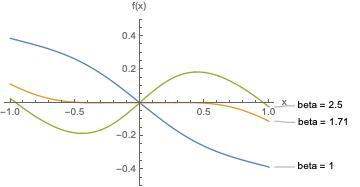
\includegraphics[width=8cm]{grafico_f.jpg}   
\caption{Plot of the function $f(x)$ for $\varepsilon = 0.5$, $\gamma =1$. The parameter $\beta$ takes three different values, $\beta = 1$, prior to the pitchfork bifurcation, $\beta = 1.71$ which is approximately the value $\beta^*_c$ for which the pitchfork bifurcation arises, and $\beta = 2.5$.}   
\label{grafico_f_subcritic}   
\end{figure}   
The critical value of the parameter $\beta$ is in this case $\beta^*_c \approx 1.714$. As we see from the plot, for subcritical values of the parameters we have only one equilibrium, corresponding to the disordered state. Then, we see the appearance of two equilibria of ferromagnetic type in $\beta^*_c$. From the linear analysis performed above, we know that - at least locally - the disordered state is stable until $\beta^{*}_c$, where it inverts its stability, with the two emerging polarized equilibria being stable. 

The case $\varepsilon \gamma > 1$ is substantially different and richer. For clarity we have divided the plots in two, fixing in both $\varepsilon = 0.5$ and $\gamma = 7$. In Figure \ref{grafico_f_super1}, it is shown that for $\beta < 2$ only the equilibrium corresponding to the disordered state is present. In $\beta = a_c \approx 2$ two other equilibria emerge, each of which then splits into two other equilibria, resulting in a total of five fixed points for the dynamics. We remark that the critical value $a_c$ at which the other two equilibria emerge was not found through the linear analysis on the bifurcations we performed above: it is indeed a global phenomenon, as the plot suggests.
Figure \ref{grafico_f_super2} shows other three values of the parameter $\beta$. In $\beta = 3$ the five equilibria are still all present, but we see that the two intermediate ones are decreasing towards $0$. Indeed, in $\beta = \beta^{*}_c \approx 5.14$ the two intermediate equilibria disappear by collapsing at $0$. This value of $\beta$ is the one corresponding to the pitchfork bifurcation we found above. Finally, in $\beta = 7$ we have three equilibria remaining: the disordered state and two polarized equilibria.

\begin{figure}   
\centering   
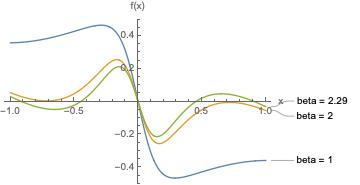
\includegraphics[width=8cm]{grafico_f_over1.jpg}   
\caption{Plot of the function $f(x)$ for $\varepsilon = 0.5$, $\gamma =7$. The parameter $\beta$ takes three different values, $\beta = 1$, $\beta = 2$ for which we see the appearance of other two equilibria, and $\beta = 2.5$ where the equilibria have become five in total.}   
\label{grafico_f_super1}   
\end{figure}   



\begin{figure}   
\centering   
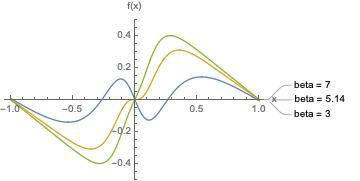
\includegraphics[width=8cm]{grafico_f_over2.jpg}   
\caption{Plot of the function $f(x)$ for $\varepsilon = 0.5$, $\gamma =7$. The parameter $\beta$ takes three different values, $\beta = 3$, where the five equilibria are still present, $\beta = 5.14$ which is approximately the value $\beta^*_c$ for which the pitchfork bifurcation arises, and $\beta = 7$, where only three equilibria survive.}   
\label{grafico_f_super2}   
\end{figure}   

\subsection{Numerical linear analysis on the other equilibria}
Even though the zeros of the function $f(x)$ cannot be found analytically, we can approximate them numerically with arbitrary precision for any choice of the parameters $\varepsilon, \gamma$ and $\beta$. The corresponding values of $y$ and $w$ can be then retrieved from the expressions in \eqref{eqn:rel}. We observe that $f(x)$ is an odd function of $x$, the same holds for the expression of $y$ in terms of $x$ in \eqref{eqn:rel}, while $w$ is even in $x$. Moreover, we remark that $x$ and $y$ at the equilibria have always opposite signs (except, trivially at the disordered one). 
Thus, denoting with $(x^-_{\varepsilon, \gamma, \beta}, y^-_{\varepsilon,\gamma,\beta},w^-_{\varepsilon,\gamma,\beta})$ the ferromagnetic polarized equilibrium with $x^-_{\varepsilon, \gamma, \beta} < 0$, we have that the corresponding positive one is $(x^+_{\varepsilon, \gamma, \beta}, y^+_{\varepsilon,\gamma,\beta},w^+_{\varepsilon,\gamma,\beta}) = (-x^-_{\varepsilon, \gamma, \beta}, -y^-_{\varepsilon,\gamma,\beta},w^-_{\varepsilon,\gamma,\beta})$.
The other two intermediate equilibria appearing for $\varepsilon \gamma > 1$ for certain values of $\beta$ are denoted with $(x^{*,-}_{\varepsilon, \gamma, \beta}, y^{*,-}_{\varepsilon,\gamma,\beta},w^{*,-}_{\varepsilon,\gamma,\beta})$ and $(x^{*,+}_{\varepsilon, \gamma, \beta}, y^{*,+}_{\varepsilon,\gamma,\beta},w^{*,+}_{\varepsilon,\gamma,\beta})$, for which of course we have again $(x^{*,+}_{\varepsilon, \gamma, \beta}, y^{*,+}_{\varepsilon,\gamma,\beta},w^{*,+}_{\varepsilon,\gamma,\beta}) = (-x^{*,-}_{\varepsilon, \gamma, \beta}, -y^{*,-}_{\varepsilon,\gamma,\beta},w^{*,-}_{\varepsilon,\gamma,\beta})$

In order to (locally) characterize the nature of these equilibria, we compute the Jacobian of the vector field in \eqref{eqn:limit_ode} at the roots of $f(x) = 0$ found numerically and the corresponding values of $y$ and $w$. 
The results obtained are the following:
\begin{itemize}
\item for $\varepsilon \gamma < 1$, the two polarized equilibria $(x^\pm_{\varepsilon, \gamma, \beta}, y^\pm_{\varepsilon,\gamma,\beta},w^\pm_{\varepsilon,\gamma,\beta})$ which emerge after the pitchfork bifurcation at $\beta^*_c$ are stable (at least locally);
\item for $\varepsilon \gamma > 1$: 
\begin{enumerate}
\item for the range of $\beta$'s where the intermediate equilibria  $(x^{*,\pm}_{\varepsilon, \gamma, \beta}, y^{*,\pm}_{\varepsilon,\gamma,\beta},w^{*,\pm}_{\varepsilon,\gamma,\beta})$ exist ($a_c < \beta < \beta^{*}_c$), they are (locally) unstable, with the Jacobian having two negative eigenvalues and a positive one;
\item the two polarized equilibria $(x^\pm_{\varepsilon, \gamma, \beta}, y^\pm_{\varepsilon,\gamma,\beta},w^\pm_{\varepsilon,\gamma,\beta})$ emerging for $ \beta > a_c$ are always (locally) stable.
\end{enumerate}
\end{itemize}

\subsection{Simulations and vector field projections}
To investigate further on the global phase portrait, and particularly on the emergence of the cycle, we performed several simulations of system \eqref{eqn:limit_ode}. Here, we restrict the parameters' values to the more interesting case $\varepsilon \gamma > 1$. In particular, we fix $\varepsilon = 0.5$ and $\gamma = 7$ from now on, in order to compare exactly the various plots.
Figures \ref{grafico_sol_b=1}, \ref{grafico_sol_b=b**}, \ref{grafico_sol_b=2.8}, and \ref{grafico_sol_b=2.9} show what happens when starting the dynamics close to the disordered state. For small values of $\beta$ (Figure  \ref{grafico_sol_b=1}) the disordered state attracts the trajectories, for $\beta \approx \beta^{**}_c$ (Figure \ref{grafico_sol_b=b**}), the value of the Hopf bifurcation, we see the emergence of periodic orbits, whose amplituted starts from small values and then expands up to $\beta = 2.8$ (Figure \ref{grafico_sol_b=2.8}), which is approximately the point where the amplitude of oscillations is maximal, since for $\beta = 2.9$ (Figure \ref{grafico_sol_b=2.9}) the periodic orbits disappear and everything gets attracted to the polarized equilibria.

\begin{figure}   
\centering   
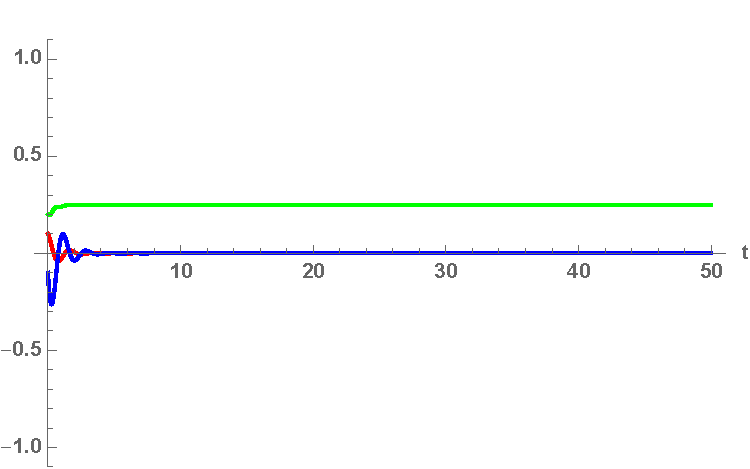
\includegraphics[width=7cm]{ode_1d_b=1.pdf}   
\caption{Plot of the solution $(x(t),y(t),w(t))$ of system \eqref{eqn:limit_ode} for $t \in [0,50]$, starting close to the disordered state, $(x(0),y(0),w(0)) = (0.1,-0.1,0.2)$, for $\beta = 1$, $\varepsilon = 0.5$ and $\gamma = 7$. The red curve is $x(t)$, the blue one is $y(t)$ and the green is $w(t)$.}   
\label{grafico_sol_b=1}   
\end{figure}   

\begin{figure}   
\centering   
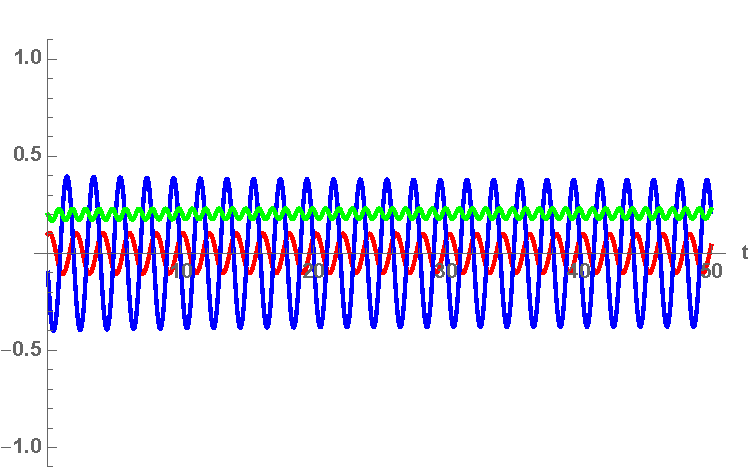
\includegraphics[width=7cm]{ode_1d_b=b**.pdf}   
\caption{Plot of the solution $(x(t),y(t),w(t))$ of system \eqref{eqn:limit_ode} for $t \in [0,50]$, starting close to the disordered state, $(x(0),y(0),w(0)) = (0.1,-0.1,0.2)$ for $\beta = 2.3 \approx \beta^{**}_c$, $\varepsilon = 0.5$ and $\gamma = 7$. The red curve is $x(t)$, the blue one is $y(t)$ and the green is $w(t)$.}   
\label{grafico_sol_b=b**}   
\end{figure}   

\begin{figure}   
\centering   
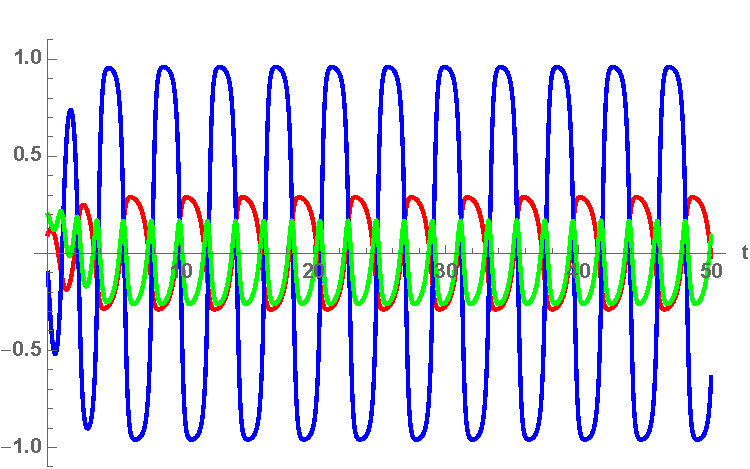
\includegraphics[width=7cm]{ode_1d_b=2_8.pdf}  
\caption{Plot of the solution $(x(t),y(t),w(t))$ of system \eqref{eqn:limit_ode} for $t \in [0,50]$, starting close to the disordered state, $(x(0),y(0),w(0)) = (0.1,-0.1,0.2)$ for $\beta = 2.8$, $\varepsilon = 0.5$ and $\gamma = 7$. The red curve is $x(t)$, the blue one is $y(t)$ and the green is $w(t)$.}   
\label{grafico_sol_b=2.8}   
\end{figure}   

\begin{figure}   
\centering   
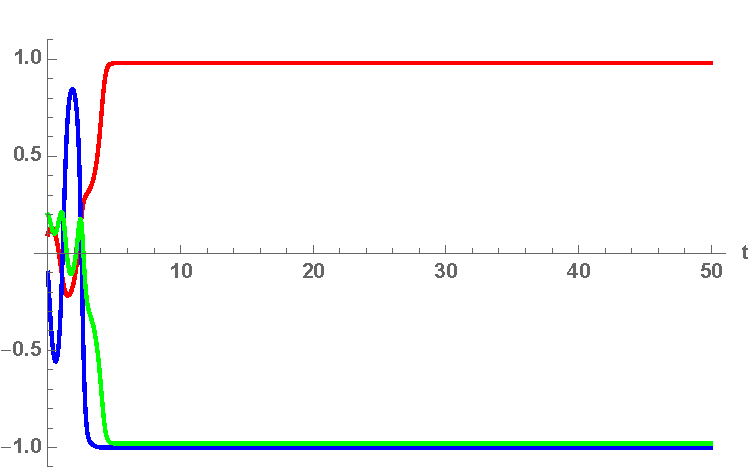
\includegraphics[width=7cm]{ode_1d_b=2_9.pdf}   
\caption{Plot of the solution $(x(t),y(t),w(t))$ of system \eqref{eqn:limit_ode} for $t \in [0,50]$, starting close to the disordered state, $(x(0),y(0),w(0)) = (0.1,-0.1,0.2)$ for $\beta = 2.9$, $\varepsilon = 0.5$ and $\gamma = 7$. The red curve is $x(t)$, the blue one is $y(t)$ and the green is $w(t)$.}   
\label{grafico_sol_b=2.9}   
\end{figure}   

\begin{figure}   
\centering   
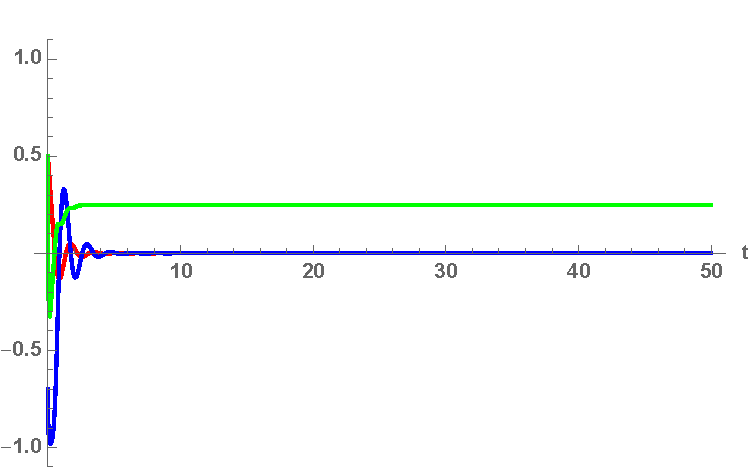
\includegraphics[width=7cm]{ode_1d_b=1_lontano.pdf}   
\caption{Plot of the solution $(x(t),y(t),w(t))$ of system \eqref{eqn:limit_ode} for $t \in [0,50]$, starting far from the disordered state, $(x(0),y(0),w(0)) = (0.5,-0.7,0.5)$ for $\beta = 1$, $\varepsilon = 0.5$ and $\gamma = 7$. The red curve is $x(t)$, the blue one is $y(t)$ and the green is $w(t)$.}   
\label{grafico_sol_b=1_lon}   
\end{figure}   

\begin{figure}   
\centering   
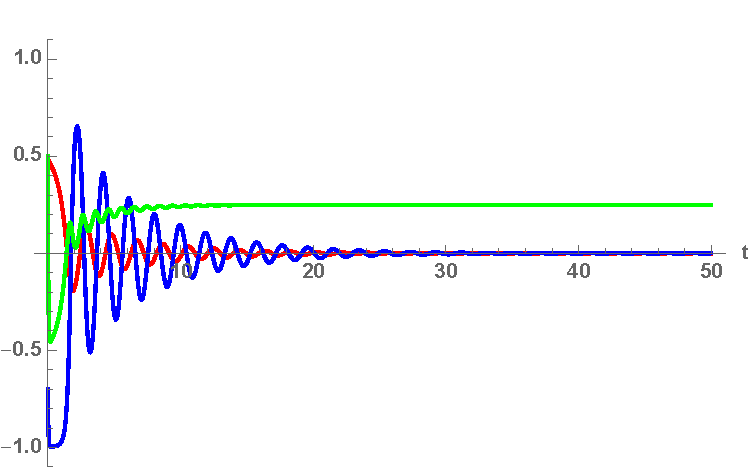
\includegraphics[width=7cm]{ode_1d_b=2_1_lontano.pdf}   
\caption{Plot of the solution $(x(t),y(t),w(t))$ of system \eqref{eqn:limit_ode} for $t \in [0,50]$, starting far from the disordered state, $(x(0),y(0),w(0)) = (0.5,-0.7,0.5)$ for $\beta = 2.1$, $\varepsilon = 0.5$ and $\gamma = 7$. The red curve is $x(t)$, the blue one is $y(t)$ and the green is $w(t)$.}   
\label{grafico_sol_b=2.1_lon}   
\end{figure}   


\begin{figure}   
\centering   
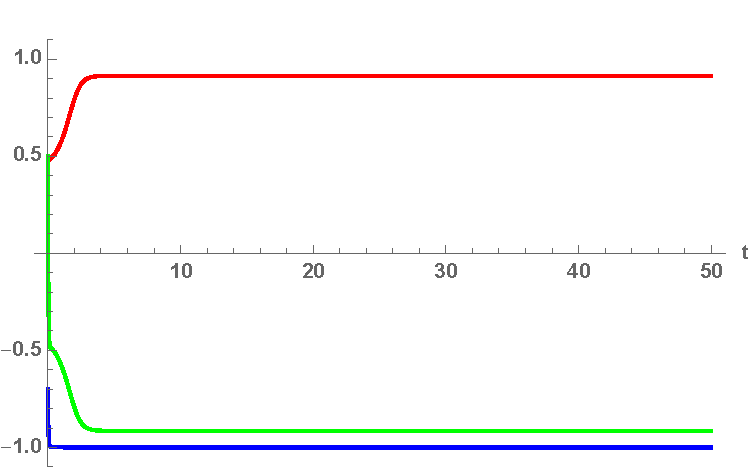
\includegraphics[width=7cm]{ode_1d_b=2_3_lontano.pdf}   
\caption{Plot of the solution $(x(t),y(t),w(t))$ of system \eqref{eqn:limit_ode} for $t \in [0,50]$, starting far from the disordered state, $(x(0),y(0),w(0)) = (0.5,-0.7,0.5)$ for $\beta = 2.3$, $\varepsilon = 0.5$ and $\gamma = 7$. The red curve is $x(t)$, the blue one is $y(t)$ and the green is $w(t)$.}   
\label{grafico_sol_b=2.3_lon}   
\end{figure}   

The picture is different when we start the dynamics far from the disordered state, as shown in Figures \ref{grafico_sol_b=1_lon}, \ref{grafico_sol_b=2.1_lon} and \ref{grafico_sol_b=2.3_lon}. As before, for small values of $\beta$ the disordered state is a global attractor for the dynamics (Figure \ref{grafico_sol_b=1_lon}); for intermediate values of $\beta$, right before the Hopf bifurcation (in Figure \ref{grafico_sol_b=2.1_lon} we considered for example $\beta = 2.1$, where here $\beta^{**}_c \approx 2.285$), the system starts to oscillate, expecially in the $y$ variable, but does not manage to reach periodic configurations before getting attracted to the polarized equilibria for values right above $\beta^{**}_c$: see Figure \ref{grafico_sol_b=2.3_lon} for the case $\beta = 2.3$.

Summing up, these pictures highlight the global attractiveness for small values of $\beta$ of the disordered state, the global attractiveness of the polarized states for big enough values of $\beta$, and the local nature of the presence of the stable cycle, which is visible only by starting the dynamics close to the disordered state, and for an intermediate range of values of $\beta$. Moreover, we have found another critical point, which we call $z_c$, where the cycle disappears. For the chosen numerical values $\varepsilon = 0.5$ and $\gamma = 7$, we find $z_c \approx 2.817$. An interesting problem is to study the way in which the cycle disappears: the fact that the cycle's amplitude increases with $\beta$, and the presence of the intermediate equilibria which at the same time get closer and closer to the disordered state, strongly suggest that the point $z_c$ could be identified as the value of $\beta$ in which the cycle falls onto the stable manifold of one of the hyperbolic intermediate equilibria. This is indeed what is happening. 

\begin{figure}   
\centering   
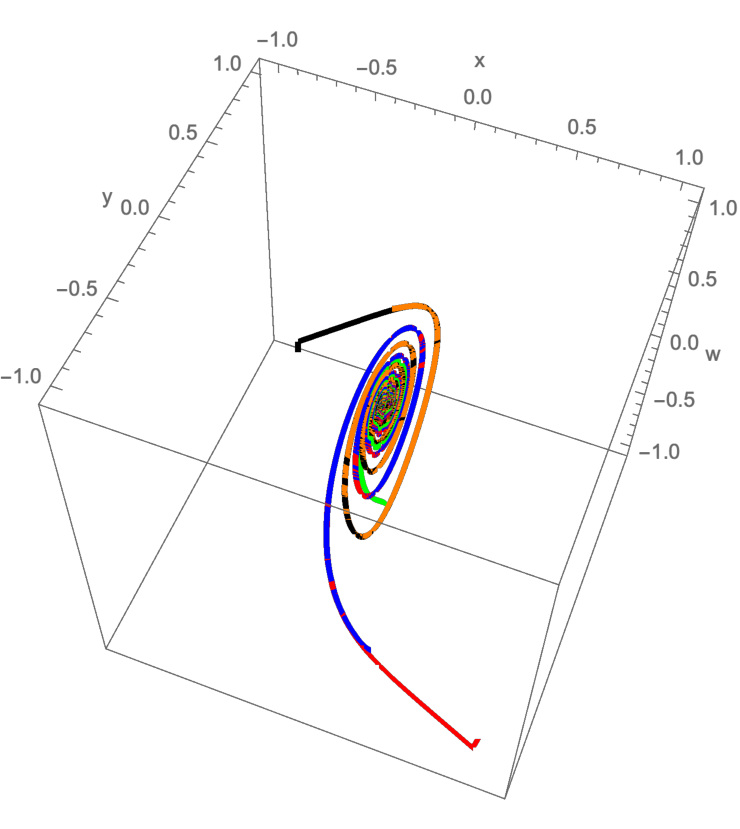
\includegraphics[width=7cm]{3D_sim_b=2.pdf}   
\caption{Parametric three-dimensional plot of trajectories starting at different inital points, for $\beta = 1.9$, right below the point where the other four equilibria appear.}   
\label{3D_pic}   
\end{figure}   


\begin{figure}   
\centering   
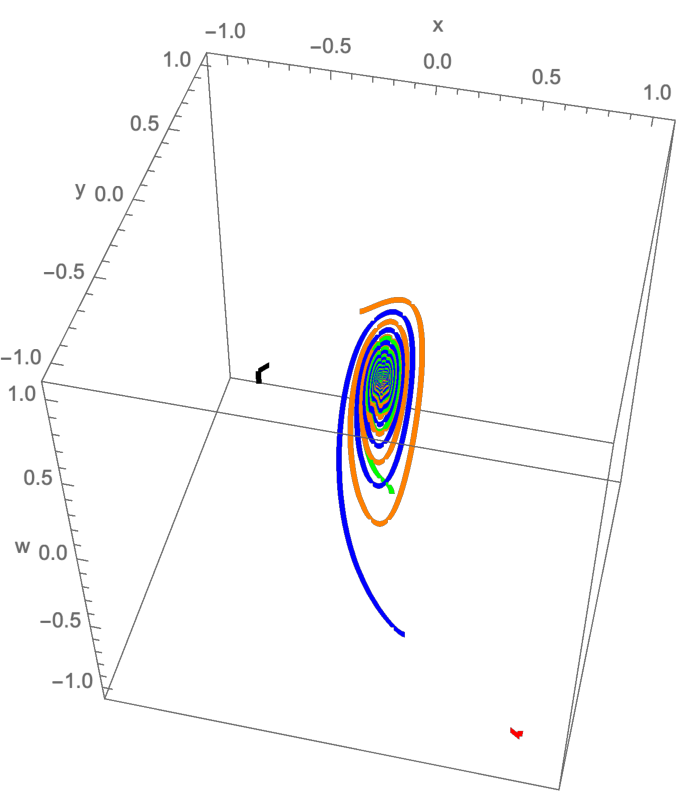
\includegraphics[width=7cm]{3D_sim_b=2_1.pdf}   
\caption{Parametric three-dimensional plot of trajectories starting at different inital points, for $\beta = 2.1$, i.e. right after the appearance of the other four equilibria.}   
\label{3D_pic1}   
\end{figure}   


\begin{figure}   
\centering   
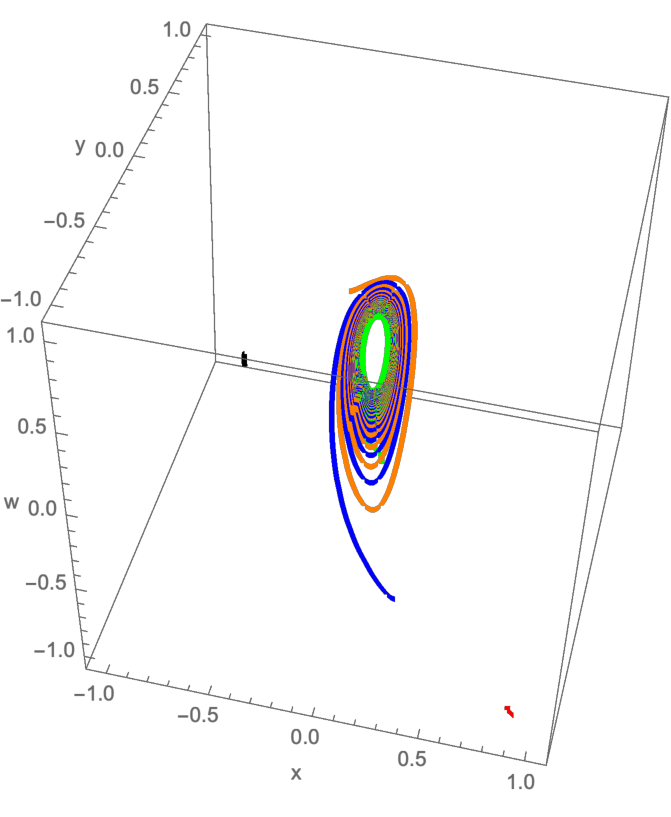
\includegraphics[width=7cm]{3D_sim_b=2_3.pdf}   
\caption{Parametric three-dimensional plot of trajectories starting at different inital points, for $\beta = 2.3$, right after the value of $\beta$ of the Hopf bifurcation.}   
\label{3D_pic2}   
\end{figure}   

\begin{figure}   
\centering   
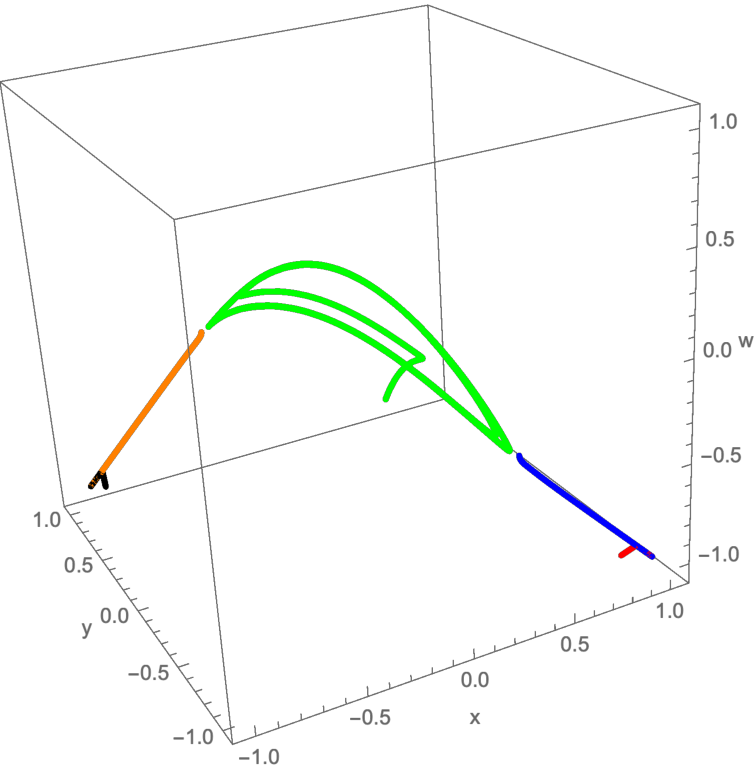
\includegraphics[width=7cm]{3D_sim_b=2_8.pdf}   
\caption{Parametric three-dimensional plot of trajectories starting at different inital points, for $\beta = 2.8$, i.e. right below the critical point $z_c$ where the periodic cycle disappears.}   
\label{3D_pic3}   
\end{figure}   

\begin{figure}   
\centering   
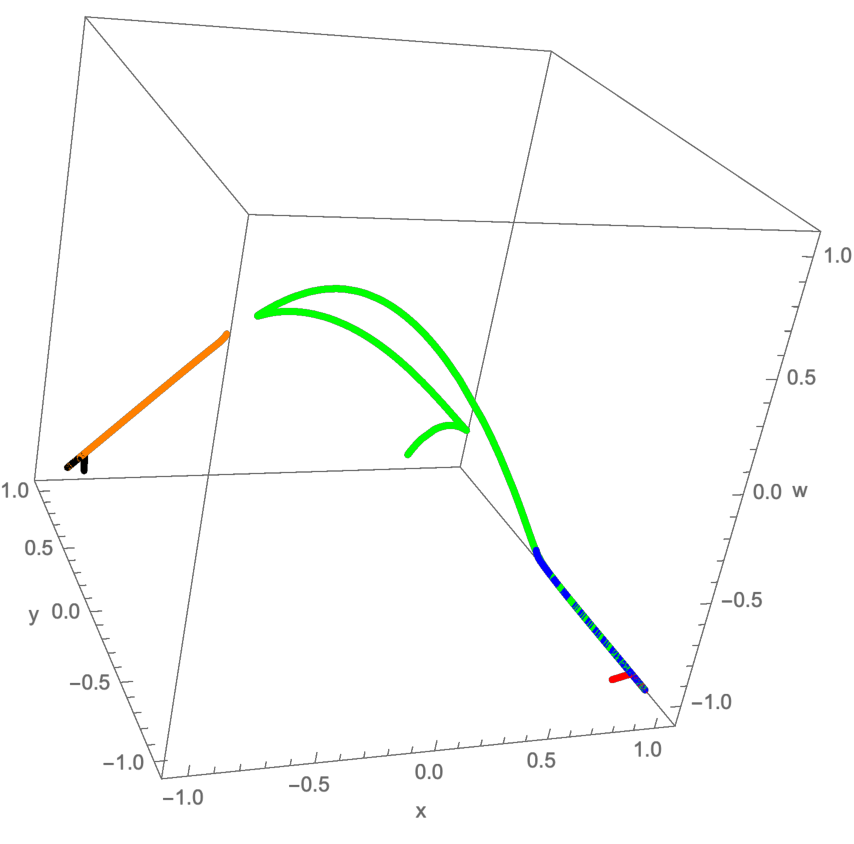
\includegraphics[width=7cm]{3D_sim_b=2_9.pdf}   
\caption{Parametric three-dimensional plot of trajectories starting at different inital points, for $\beta = 2.9$, i.e. right above the critical point $z_c$ where the periodic cycle disappears.}   
\label{3D_pic4}   
\end{figure}   

\begin{figure}   
\centering   
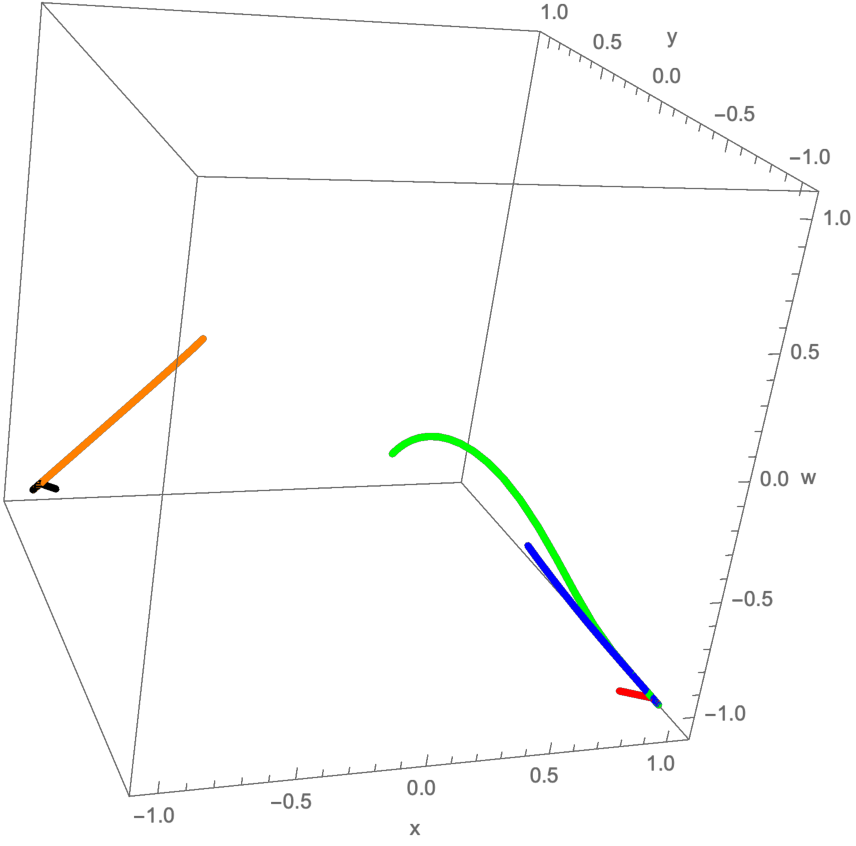
\includegraphics[width=7cm]{3D_sim_b=5_3.pdf}   
\caption{Parametric three-dimensional plot of trajectories starting at different inital points, for $\beta = 5.3$, where the unstable intermediate equilibria have disappeared, and the polarized equilibria remain the only attractive equilibria in the dynamics.}   
\label{3D_pic5}   
\end{figure}   

In Figures \ref{3D_pic}, \ref{3D_pic1}, \ref{3D_pic2}, \ref{3D_pic3}, \ref{3D_pic4} and \ref{3D_pic5} we show some parametric three-dimensional plots of five trajectories of system \eqref{eqn:limit_ode}, produced by starting the dynamics on different initial points, focusing on values of $\beta$ around $a_c$, $\beta^{**}_c$, $z_c$ and $\beta^*_c$. The trajectory in green was obtained by starting close to the disordered state, the blue and the orange ones in an intermediate state, while the red and the black trajectories are starting close to the polarized states. 
We see that, for values of $\beta < a_c$ (Figure \ref{3D_pic}), the disordered state attracts all the five trajectories, and it is a focus.
When increasing $\beta$ right above the value $a_c$ where the other four equilibria appear, we see that (Figure \ref{3D_pic1}) the red and black solutions are now well distinguished and tend towards the polarized states closer to them, while the solutions in blue and orange, which started close to the unstable intermediate equilibria, get still attracted to the disordered state. Of course, if we started these two solutions closer to the polarized states we would have seen an attraction towards the other equilibria. 
In Figure \ref{3D_pic2} we have chosen a $\beta$ right above the critical value $\beta^{**}_c$ of the Hopf bifurcation: we here indeed see the appearance of a cycle (the one in green), and that the two intermediate solutions get attracted to the cycle.
The cycle increases its amplitude until $\beta \approx 2.8$, which is shown in Figure \ref{3D_pic3}.  Here, even though the cycle is still stable, the two intermediate solutions in orange and blue are now attracted to the polarized states: indeed, the actual value of the unstable intermediate equilibria is decreasing towards the disordered state as $\beta$ increases, but we are keeping fixed the initial "intermediate" data so that after a while it falls within the domain of attraction of the extreme equibria.
\begin{figure}   
\centering   
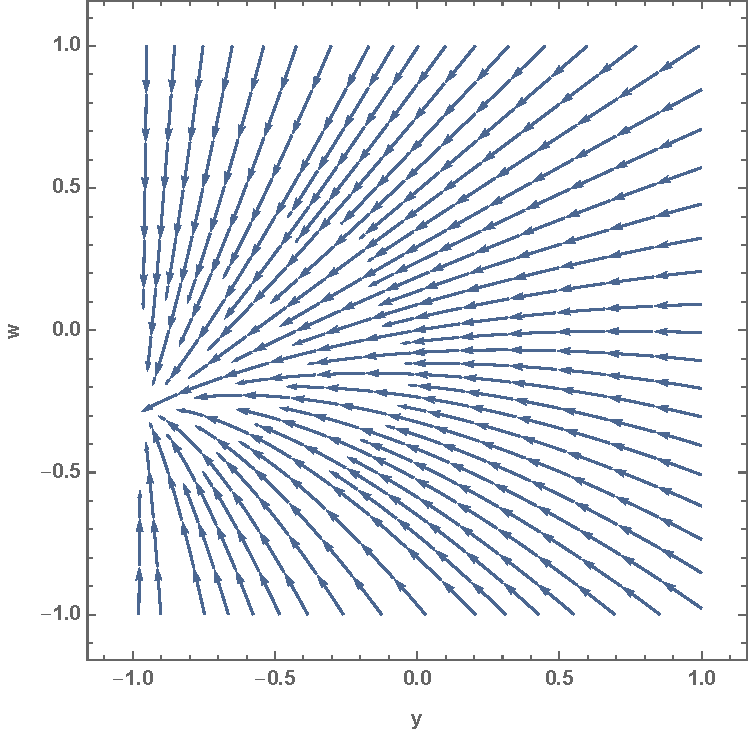
\includegraphics[width=6cm]{stream_x.pdf}   
\caption{The vector field projected onto the plane $x = \bar{x} \approx x^{*,+}_{\varepsilon, \gamma, \beta}$ for $\beta = 2.8$.}
\label{stream_x}   
\end{figure}   

\begin{figure}   
\centering   
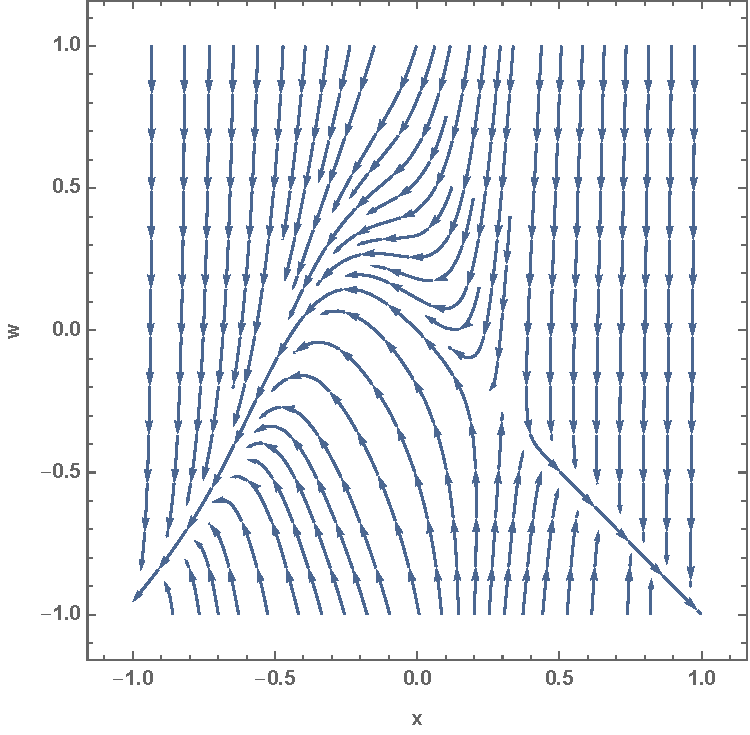
\includegraphics[width=6cm]{stream_y.pdf}   
\caption{The vector field projected onto the plane $y = \bar{y} \approx y^{*,-}_{\varepsilon,\gamma,\beta}$ for $\beta = 2.8$.}   
\label{stream_y}   
\end{figure}   

\begin{figure}   
\centering   
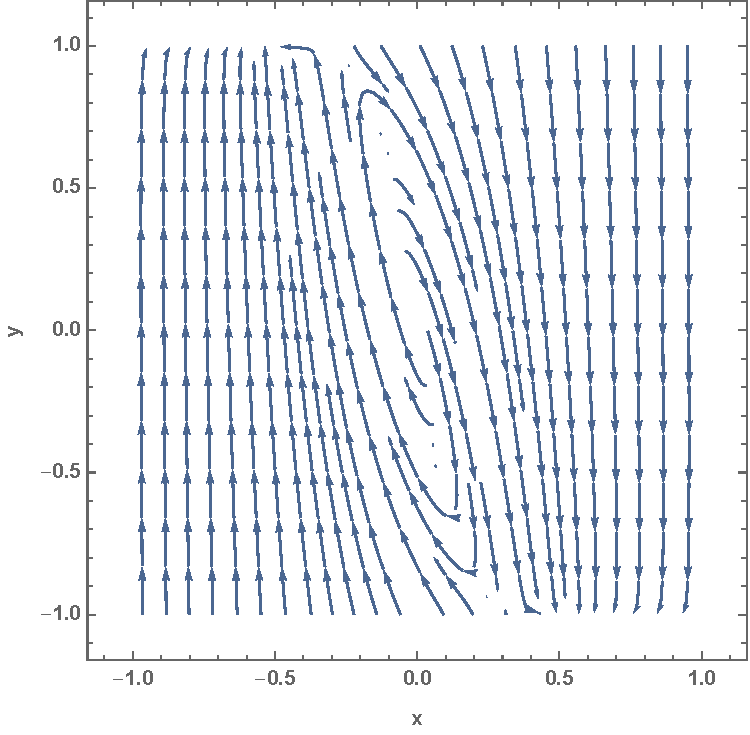
\includegraphics[width=6cm]{stream_w.pdf}   
\caption{The vector field projected onto the plane $w = \bar{w} \approx w^{*,-}_{\varepsilon,\gamma,\beta}$ for $\beta = 2.8$.}   
\label{stream_w}   
\end{figure}   
Figure \ref{3D_pic4} was realized by choosing a $\beta$ right above the critical value $z_c$ where the cycle disappears: as expected, the trajectory in green touches one of the two intermediate solutions (in this case the red one), and consequently gets attracted towards the polarized state. As we saw from the linear analysis around the intermediate equilibria, we know that locally we have a two dimensional stable manifold and a one dimensional unstable one. Necessarily then, the cycle eventually hits the two dimensional stable manifold, the resulting trajectory escapes through the one dimensional unstable curve, and finally it gets attracted to the polarized state. A confirmation of this is shown in Figures \ref{stream_x}, \ref{stream_y}, \ref{stream_w}, where we plotted the vector field projected onto the three coordinates $x$, $y$ and $w$, for a value of $\beta$ right below $z_c$. As we see from the pictures, the plane $x = \bar{x} \approx x^{*,+}_{\varepsilon, \gamma, \beta}$ is (approximately) the stable two dimensional manifold associated to the intermediate equilibrium.



Figure \ref{3D_pic5} finally shows the three-dimensional simulation for a big value of $\beta$, after the pitchfork bifurcation in $\beta^*_c$ where the two intermediate unstable equilibria vanish. Here, the green trajectory oscillates less and less and gets attracted to the polarized state, which is the only stable equilibrium in the dynamics and thus attracts all the trajectories.







\begin{thebibliography}{9}

\bibitem{perko}
L. Perko.
\newblock Differential Equations and Dynamical Systems.
\newblock \emph{Texts in Applied Mathematics 7}, Third Edition, 2001.

\end{thebibliography}



\end{document}


